%Preamble
\documentclass[12pt]{article}
\usepackage{fancyhdr}
\usepackage{extramarks}
\usepackage{amsmath}
\usepackage{amssymb}
\usepackage{amsthm}
\usepackage{amsrefs}
\usepackage{amsfonts}
\usepackage{mathrsfs}
\usepackage{mathtools}
\usepackage[mathcal]{eucal} %% changes meaning of \mathcal
\usepackage{enumerate}
\usepackage[shortlabels]{enumitem}
\usepackage{verbatim} %% includes comment environment
\usepackage{hyperref}
\usepackage[capitalize]{cleveref}
\crefformat{equation}{~(#2#1#3)}
\usepackage{caption, subcaption}
\usepackage{graphicx}
\usepackage{fullpage} %%smaller margins
\usepackage[all,arc]{xy}
\usepackage{mathrsfs}

\hypersetup{
    linktoc=all,     % set to all if you want both sections and subsections linked
}

\topmargin=-0.45in
\evensidemargin=0in
\oddsidemargin=0in
\textwidth=6.5in
\textheight=9.0in
\headsep=0.25in
\setlength{\headheight}{16pt}

\linespread{1.0}

\pagestyle{fancy}
\lhead{\Name}
\chead{\hwClass: \hwTitle}
\rhead{\hwDueDate}
\lfoot{\lastxmark}
\cfoot{\thepage}

\renewcommand\headrulewidth{0.4pt}
\renewcommand\footrulewidth{0.4pt}

\setlength\parindent{0pt}

%% Title Info
\newcommand{\hwTitle}{HW \# 2}
\newcommand{\hwDueDate}{Jan 22, 2020}
\newcommand{\hwClass}{AMATH 585}
\newcommand{\hwClassTime}{}
\newcommand{\hwClassInstructor}{}
\newcommand{\Name}{\textbf{Marlin Figgins}}


%% MATH MACROS
\newcommand{\bbF}{\mathbb{F}}
\newcommand{\bbN}{\mathbb{N}}
\newcommand{\bbQ}{\mathbb{Q}}
\newcommand{\bbR}{\mathbb{R}}
\newcommand{\bbZ}{\mathbb{Z}}
\newcommand{\bbC}{\mathbb{C}}
\newcommand{\abs}[1]{ \left| #1 \right| }
\newcommand{\diff}[2]{\frac{d #1}{d #2}}
\newcommand{\infsum}[1]{\sum_{#1}^{\infty}}
\newcommand{\norm}[1]{ \left|\left| #1 \right|\right| }
\newcommand{\eval}[1]{ \left. #1 \right| }
\newcommand{\Expect}[1]{\mathbb{E}\left[#1 \right]}
\newcommand{\Var}[1]{\mathbb{V}\left[#1 \right]}
\renewcommand{\vec}[1]{\mathbf{#1}}

\renewcommand{\phi}{\varphi}
\renewcommand{\emptyset}{\O}

%--------Theorem Environments--------
%theoremstyle{plain} --- defaultx
\newtheorem{thm}{Theorem}[section]
\newtheorem{cor}[thm]{Corollary}
\newtheorem{prop}[thm]{Proposition}
\newtheorem{lem}[thm]{Lemma}
\newtheorem{conj}[thm]{Conjecture}
\newtheorem{quest}[thm]{Question}

\theoremstyle{definition}
\newtheorem{defn}[thm]{Definition}
\newtheorem{defns}[thm]{Definitions}
\newtheorem{con}[thm]{Construction}
\newtheorem{exmp}[thm]{Example}
\newtheorem{exmps}[thm]{Examples}
\newtheorem{notn}[thm]{Notation}
\newtheorem{notns}[thm]{Notations}
\newtheorem{addm}[thm]{Addendum}

% Environments for answers and solutions
\newtheorem{exer}{Exercise}
\newtheorem{sol}{Solution}

\theoremstyle{remark}
\newtheorem{rem}[thm]{Remark}
\newtheorem{rems}[thm]{Remarks}
\newtheorem{warn}[thm]{Warning}
\newtheorem{sch}[thm]{Scholium}

\makeatletter
\let\c@equation\c@thm
\makeatother

\begin{document}
\begin{exer}
 (Inverse matrix and Green's functions)
\begin{enumerate}
\item Write out the $4\times 4$
matrix $A$ from (2.43) for the boundary value problem
$u''(x)=f(x)$ with $u(0)=u(1)=1$ and for  $h = 1/3$.

\item Write out the $4\times 4$
inverse matrix $A^{-1}$ explicitly for this problem.

\item
If $f(x)=x$, determine the discrete approximation to the solution of the
boundary value problem on this grid and sketch this solution and the four
Green's functions from which the solution is obtained.  (You may use Matlab or
other tools for plotting, or you may plot by hand.)
\end{enumerate}
\end{exer}

\begin{sol}
    (a) Using equation (2.43) as a guide, we can write out the matrix $A$ as 
\begin{align*}
A = 9
\begin{pmatrix}
    \frac{1}{9} & 0 & 0 & 0 \\
1 & -2 & 1 & 0\\
0 & 1 & -2 & 1\\
0 & 0 & 0 & \frac{1}{9}
\end{pmatrix}
\end{align*}

(b)  We'll use a grid of points
\begin{equation*}
x_{0} = 0, x_{1} = \frac{1}{3}, x_{2} = \frac{2}{3}, x_{3} = 1.
\end{equation*}

As shown in class the matrix $A^{-1} = B$ has elements
\begin{align*}
    B_{i+1,j+1} = h G(x_{i}, x_{j}) 
    = \begin{cases}
        \frac{x_{i}}{3} (x_{j}-1) \ \quad i < j \\
        \frac{x_{j}}{3} (x_{i}-1) \ \quad i \geq j 
    \end{cases},
\end{align*}
with the exception of the first and last columns given by $G_{0}(x) = 1 - x$ and $G_{1}(x) = x$ respectively.
Using Julia for a bit of assistance, we see the full matrix is 

\begin{align*}
A^{-1} = B = 
\begin{pmatrix}
   1 & 0 & 0 & 0\\
   \frac{2}{3} & -\frac{2}{27}& -\frac{1}{27}&  \frac{1}{3}\\
   \frac{1}{3} & -\frac{1}{27} & -\frac{2}{27} & \frac{2}{3}\\
   0 & 0 & 0 & 1
\end{pmatrix}.
\end{align*}

(c) When $f(x) = x$, our solution $U$ is determined by
\begin{align*}
\begin{pmatrix}
    U_{0}\\
    U_{1}\\
    U_{2}\\
    U_{3}
\end{pmatrix} = A^{-1} 
\begin{pmatrix}
    1\\
    \frac{1}{3}\\
    \frac{2}{3}\\
    1
\end{pmatrix} 
\end{align*}

We implement this method of solving the BVP in julia and plot the Green's functions and the approximations below.


\end{sol}




\begin{figure}[ht]
    \centering
    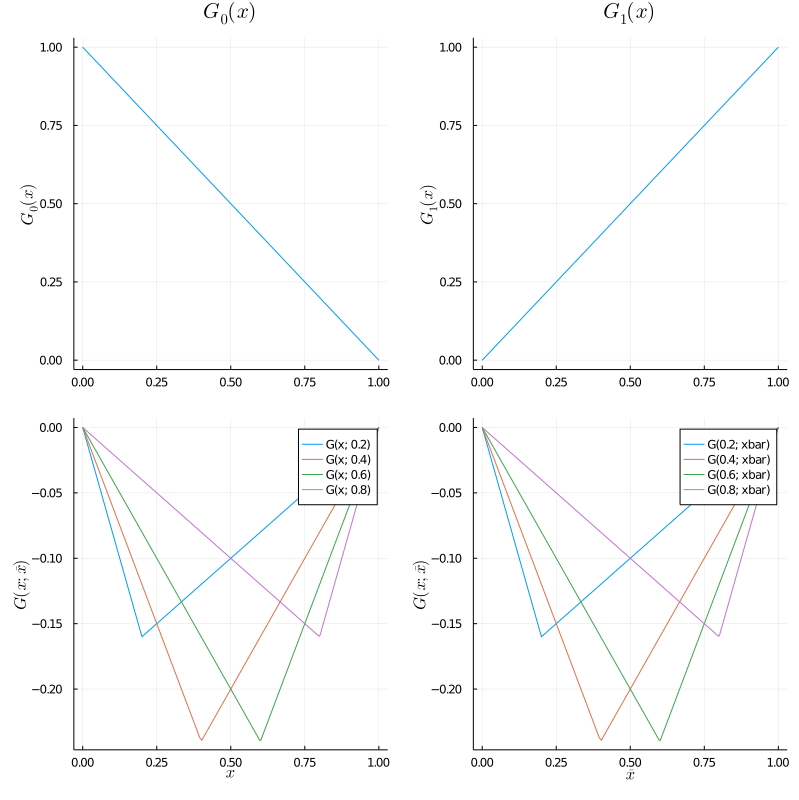
\includegraphics[width=0.7\linewidth]{figs/hw-2-greens-plot.png}
    \caption{Plotting relevant Green's Functions}%
    \label{fig:figs/}
\end{figure}

\begin{figure}[ht]
    \centering
    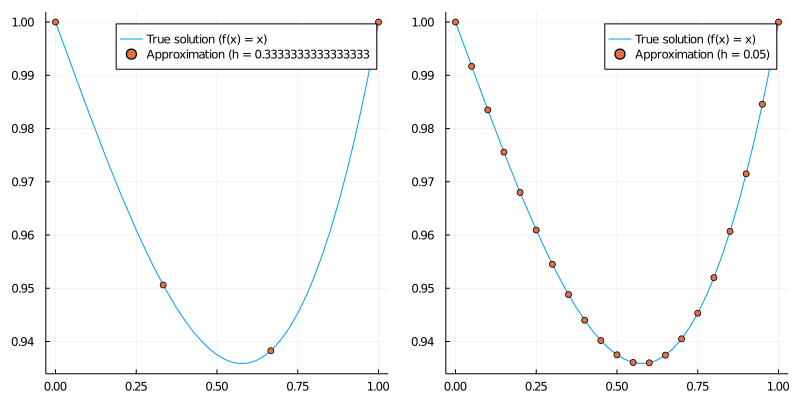
\includegraphics[width=0.7\linewidth]{figs/hw-2-approx-plot.png}
    \caption{Plotting approximate solutions $\hat{u}(x)$  for $h = \frac{1}{4}$ and $h=\frac{1}{20}$.}
    \label{fig:figs/hw-2-approx-plot}
\end{figure}

\newpage

\

\newpage

\

\newpage

\begin{exer}
(Another way of analyzing the error using Green's functions)
The {\em composite trapezoid rule} for integration approximates the
integral from $a$ to $b$ of a function $g$ by dividing the interval
into segments of length $h$ and approximating the integral over each
segment by the integral of the linear function that matches $g$ at
the endpoints of the segment. (For $g > 0$, this is the area of
the trapezoid with height $g( x_j )$ at the left endpoint $x_j$
and height $g( x_{j+1} )$ at the right endpoint $x_{j+1}$.)  Letting
$h = (b-a)/(m+1)$ and $x_j = a + jh$, $j = 0,1, \ldots , m, m+1$:
\[
\int_a^b g(x)\,dx \approx  h \sum_{j=0}^m \frac{g( x_j )+g( x_{j+1} )}{2} 
     =  h \left[ \frac{g( x_0 )}{2} + \sum_{j=1}^m g( x_j ) + 
                   \frac{g( x_{m+1} )}{2} \right] .
\]

\begin{enumerate}
\item
Assuming that $g$ is sufficiently smooth, show that the error in the 
composite trapezoid rule approximation to the integral is $O( h^2 )$.
[Hint:  Show that the error on each subinterval is $O( h^3 )$.]

\item
Recall that the true solution of the boundary value problem $u'' (x) = f(x)$,
$u(0) = u(1) = 0$ can be written as
\begin{equation}
u(x) = \int_0^1 f( \bar{x} ) G(x; \bar{x} )\,d \bar{x} , \label{1}
\end{equation}
where $G(x; \bar{x})$ is the Green's function corresponding to
$\bar{x}$.  The finite difference approximation $u_i$ to $u( x_i )$, 
using the centered finite difference scheme in (2.43), is
\begin{equation}
u_i = h \sum_{j=1}^m f( x_j ) G( x_i ; x_j ) ,~~i=1, \ldots , m . \label{2}
\end{equation}
Show that formula (\ref{2}) is the trapezoid rule approximation to 
the integral in (\ref{1}) when $x = x_i$, and conclude from this that the 
error in the finite difference approximation is $O( h^2 )$ at each node $x_i$. 
[Recall:  The Green's function $G( x ; x_j )$ has a {\em discontinuous}
derivative at $x = x_j$.  Why does this not degrade the accuracy of the
composite trapezoid rule?]
\end{enumerate}
\end{exer}

\begin{sol}
1. Writing $g(x)$ in terms of its Taylor expansion
\begin{equation*}
    g(x) = g(x) + g'(x) h + O(h^{2})
\end{equation*}
integrating this relationship over the interval $[x, x+h]$, we have
\begin{equation*}
\int_{x}^{x+h} g(t)dt = h g(x) + \frac{h^{2}}{2} g'(x) + O(h^{3}).
\end{equation*}
Writing out the forward difference approximation for the first derivative which is $O(h)$, we see
\begin{align*}
    \frac{h^{2}}{2} g'(x) =  \frac{h}{2} ( g(x+h) - g(x)) + O(h^{3}).
\end{align*}
We then have that
\begin{align*}
    \int_{x}^{x+h} g(t)dt = \frac{h}{2} (g(x) + g(x+h)) + O(h^{3}),
\end{align*}
which shows that the error on a single subinterval of length $h$ is $O(h^{3})$. Summing this across all subintervals of which there are $(b - a )/ h$, we have that the entire error is 
\begin{align*}
    \int_{a}^{b} g(x)dx &= \sum_{i = 0}^{m+1} \int_{x_{i}}^{x_{i} + h} g(x) dx\\
                        &=\sum_{i = 0}^{m+1} \left(  \frac{h}{2} (g(x_{i}) + g(x_{i}+h)) + O(h^{3}) \right )\\
                        &= \frac{h}{2} g(x_{0}) + h \sum_{i = 1}^{m} g(x_{i}) + \frac{h}{2} g(x_{m+1}) + O(h^{2}).
\end{align*}
Therefore, the error has order $O(h^{2})$.


2. We will approximate the following integral with the composite trapezoid rule approximation
\begin{align*}
u(x_{i}) = \int_0^1 f( \bar{x} ) G(x_{i}; \bar{x} )\,d \bar{x} 
\end{align*}
Under the Trapezoid rule approximation, this becomes
\begin{align}
    u(x_{i}) &\approx \frac{h}{2} f( x_0 ) G( x_i ; x_0 ) + h \sum_{j = 1}^{m} f( x_j ) G( x_i ; x_j )  + \frac{h}{2} f( x_{m+1} ) G( x_{i} ; x_{m+1} ) \\ 
             &=  h \sum_{j = 1}^{m} f( x_j ) G( x_i ; x_j ),
\end{align}
where we've used that $G(x_{i}; 0) = 0$ and $G(x_{i}; 1) = 0$. As this is simply the trapezoid approximation of the integral, we conclude that it has order $O(h^{2})$. This holds despite the discontinuity in the derivative of $G(x ; x_{j})$ at $x = x_{j}$ due to the fact that the function is piecewise linear and its derivative is estimated using a forward difference i.e. at $x_{j}$ the function is approximating the right hand derivative which does still exist and is of order $O(h)$. Though the derivative of $G$ technically does not exist here, the error over the subinterval it contributes by using the forward difference is still of order $O(h^{3})$ and contributed once and is inconsequential as $h\to 0$. Therefore, the total order of the algorithm is not degraded. 
\end{sol}

\newpage

\begin{exer}
 (Green's function with Neumann boundary conditions)
\begin{enumerate}
\item
Determine the Green's functions for the two-point boundary
value problem $u''(x) = f(x)$ on $0<x<1$ with a Neumann boundary condition
at $x=0$ and a Dirichlet condition at $x=1$, i.e, find the function
$G(x,\bar x)$ solving
\[
u''(x) = \delta(x-\bar x), \quad u'(0)=0, \quad u(1)=0
\]
and the functions $G_0(x)$ solving
\[
u''(x) = 0, \quad u'(0)=1, \quad u(1)=0
\]
and $G_1(x)$ solving
\[
u''(x) = 0, \quad u'(0)=0, \quad u(1)=1.
\]
\item
Using this as guidance, find the general formulas for the elements of the
inverse of the matrix in equation (2.54).  Write out the $4\times 4$ matrices
$A$ and $A^{-1}$ for the case $h=1/3$.
\end{enumerate}
\end{exer}

\begin{sol}
    Starting with $G_{0}(x)$ and $G_{1}(x)$, the conditions given show that our solutions are
    \begin{align*}
        G_{0}(x) = x - 1\\
        G_{1}(x) = 1.
    \end{align*}
    Now to solve for $G(x, \overline{x})$, we know that 
    \begin{align*}
        u'(1) - u'(0) &= \int_{0}^{1} u''(x) dx \\
                      &= \int_{0}^{1} \delta(x - \overline{x}) = 1. 
    \end{align*}
    Since $u'(0) = 0$, this shows that $u'(1) = 1$. Therefore, we can write 
    \begin{align*}
        G(x; \overline{x}) = 
        \begin{cases}
            \overline{x} - 1 &\text{ for } 0 \leq x < \overline{x}\\
            x - 1 &\text{ for } \overline{x} \leq x \leq 1 
        \end{cases}
    \end{align*}
    which satisfies $G'(0; \overline{x}) = 0$, $G(1; \overline{x}) = 0$ and the second derivative condition we derived $G'(1, \overline{x}) = 1$ as well as the second derivative being 0 where it exists.


    2. We can use these functions to determine the columns of the inverse matrix. In the case of the first and last columns of our inverse matrix $A^{-1}$, we write
\begin{align*}
    (A^{-1})_{i1} = G_{0}(x_{i}) \\
    (A^{-1})_{i,m+1} = G_{1}(x_{i}) 
\end{align*}
with all other elements given by 

\begin{align*}
    (A^{-1})_{i+1,j+1} = h G(x_{i}, x_{j}).
\end{align*}
Here, entries are shifted since we index the grid points starting with 0 and the matrix with 1. Writing out the matrix $A$ explicitly, we see
\begin{align*}
A = 9
\begin{pmatrix}
    -\frac{1}{3} & \frac{1}{3} & & \\
    1 & - 2 & 1 & \\
      & 1 & -2 & 1\\
      &   &    & \frac{1}{9}
\end{pmatrix}
\end{align*}

Our Green's functions give the inverse matrix as
\begin{align*}
    A^{-1} = \begin{pmatrix}
    -1 & -\frac{2}{9} & - \frac{1}{9} & 1\\
    -\frac{2}{3} & -\frac{2}{9} & -\frac{1}{9} & 1\\
    -\frac{1}{3} & -\frac{1}{9} & - \frac{1}{9} & 1\\
    0 & 0 & 0 & 1
\end{pmatrix}
\end{align*}
\end{sol}

\newpage

\begin{exer}
 (Solvability condition for Neumann problem)
Determine the null space of the matrix $A^T$, where $A$ is given in
equation (2.58), and verify that the condition (2.62) must hold for the
linear system to have solutions.
\end{exer}

\begin{sol}
    We'll now find the nullspace of $A^{T}$ which will satisfy
    \begin{align*}
    A^{T} U = \vec{0}.
    \end{align*}
    This means that we have the following equations
    \begin{align*}
        -h U_{0} + U_{1} &= 0\\
        h U_{0} - 2 U_{1} + U_{2} &= 0\\
        U_{1} - 2U_{2} + U_{3} &= 0 \\
                                  &\vdots\\  
        U_{m-1} - 2 U_{m} + hU_{m+1} &= 0\\
        U_{m} - h U_{m+1} &= 0.
    \end{align*}
    We then have
    \begin{align*}
        hU_{0} &= U_{1}\\
        h U_{0} - 2h U_{0} + U_{2} = 0 \implies h U_{0} &= U_{2}\\
        h U_{0} - 2 h U_{0} + U_{3} = 0 \implies h U_{0} &= U_{3}\\
                                                         &\vdots \\
        h U_{0} - 2h U_{0} + U_{m} = 0 \implies   h U_{0} &= U_{m}\\
                                                    U_{0} &= U_{m+1}
    \end{align*}
    if $U$ is in the null space of $A^{T}$. This means that the nullspace is spanned by the vector
    \begin{align*}
        U = (1, h, h, \cdots, h, h, 1).
    \end{align*}
    As we know, for $A$ to have a solution, we must find vectors which are orthogonal to the nullspace of $A^{T}$. We then have that if a vector $F$ of the form in 2.58 is orthogonal to the nullspace i.e. $U \cdot F = 0$, then
    \begin{align*}
        U \cdot F &= \sigma_{0} + \frac{h}{2} f(x_{0}) + \sum_{j = 1}^{m} h f(x_{j}) +  \frac{h}{2} f(x_{m+1}) - \sigma_{1} = 0.
    \end{align*}
    Moving $\sigma_{1}$ and $\sigma_{0}$ to the other side of the equation gives the desired condition. 

\end{sol}

\newpage

\begin{exer}
 (Symmetric tridiagonal matrices)
\begin{enumerate}
\item
Consider the {\bf Second approach} described on p.~31 for dealing with
a Neumann boundary condition.  If we use this technique to approximate
the solution to the boundary value problem $u'' (x) = f(x)$, 
$0 \leq x \leq 1$, $u' (0) = \sigma$, $u(1) = \beta$, then the resulting
linear system $A {\bf u} = {\bf f}$ has the following form:
\[
\frac{1}{h^2} \left( \begin{array}{ccccc}
-h & h  &        &        &      \\
1  & -2 & 1      &        &      \\
   & 1  & \ddots & \ddots &      \\
   &    & \ddots & \ddots & 1    \\
   &    &        & 1      & -2 \end{array} \right)
\left( \begin{array}{c} u_0 \\ u_1 \\ \vdots \\ u_{m-1} \\ u_{m} \end{array} 
\right) =
\left( \begin{array}{c} \sigma + (h/2) f( x_0 ) \\ f( x_1 ) \\ \vdots \\ 
f( x_{m-1} ) \\ f( x_m ) - \beta / h^2 \end{array} \right) .
\]
Show that the above matrix is similar to a symmetric tridiagonal matrix 
via a {\em diagonal} similarity transformation; that is, there is a diagonal
matrix $D$ such that $D A D^{-1}$ is symmetric.
\item
Consider the {\bf Third approach} described on pp.~31-32 for dealing with
a Neumann boundary condition.  [{\bf Note:} If you have an older edition of the text,
there is a typo in the matrix (2.57) on p.~32.  There should be a row above what is written
there that has entries $\frac{3}{2} h$, $-2h$, and $\frac{1}{2} h$
in columns $1$ through $3$ and $0$'s elsewhere.  I believe this was corrected in newer editions.]  
Show that if we use that first equation
(given at the bottom of p. 31) to eliminate $u_0$ and we also eliminate
$u_{m+1}$ from the equations by setting it equal to $\beta$ and modifying
the right-hand side vector accordingly, then we obtain an $m$ by $m$
linear system $A {\bf u} = {\bf f}$, where $A$ is similar to a symmetric
tridiagonal matrix via a diagonal similarity transformation.
\end{enumerate}
\end{exer}

\begin{sol}
    1. Suppose we have a diagonal matrix $D$ with diagonal $(\lambda_{0}, \cdots, \lambda_{m+1})$. Then we have that
    \begin{align*}
    D A D^{-1} = 
\frac{1}{h^2} \left( \begin{array}{ccccc}
-h & h  / \lambda_{1} &        &        &      \\
1 / \lambda_{0} & -2  & 1 / \lambda_{2}      &        &      \\
   & 1 / \lambda_{1}  & \ddots & \ddots &      \\
   &    & \ddots & \ddots & 1 / \lambda_{m+1}    \\
   &    &        & 1 / \lambda_{m}     & -2 \end{array} \right)
    \end{align*}
\end{sol}
From this, we see that selecting $\lambda_{0} = 1 / h$ and all other $\lambda_{i} = 1$ should produce a symmetric matrix.


2. Using equation at bottom of pg 31, we write
\begin{align*}
U_{0} = \sigma h + \frac{4}{3}U_{1} - \frac{1}{3}U_{2},
\end{align*}
which combined with the second derivative approximation for $U''(x_{1}) = f(x_{2})$ allow us to remove the first equation and rewrite the second as
\begin{equation*}
    \frac{1}{h^{2}} \left(- \frac{2}{3} U_{1} + \frac{2}{3}U_{2}\right ) = f(x_{2}) - \frac{\sigma}{h}
\end{equation*}
Aslso eliminating the $U_{m+1}$ variable as described leaves us with the $m \times m$ matrix
\begin{align*}
A = \frac{1}{h^2} \left( \begin{array}{ccccc}
        -\frac{2}{3} & \frac{2}{3}      &   &          \\
    1  & -2 & 1 &      \\
       & \ddots & \ddots & 1    \\
       &        & 1      & -2 \end{array} \right)
\end{align*}
Based on the knowledge of diagonal similarity transforms developed in part one, we see that using a diagonal matrix with diagonal $(\frac{3}{2}, 1, \cdots, 1)$ gives the desired transform since the only `problem' element is $A_{21} = 1$.

\newpage

\end{document}
